%!TEX root = ../../thesis.tex
%*******************************************************************************
%****************************** Concept Chapter *********************************
%*******************************************************************************

\chapter{Solution Concept}

\ifpdf
    \graphicspath{{Chapters/Solution-Concept/Figs/}{Chapters/Solution-Concept/Figs/}{Chapters/Solution-Concept/Figs/}}
\else
    \graphicspath{{Chapters/Solution-Concept/Figs/}{Chapters/Solution-Concept/Figs/}}
\fi
In the previous chapter, we defined different design requirements and principles for our solution approach. 
Based on that, in this chapter, we present the conceptual design of the solution, which outlines the system's key features, components, and functionalities. 
The Solution Concept chapter in software engineering provides a comprehensive understanding of the proposed solution approach. 
This chapter bridges the gap between the solution design and the actual implementation of the solution by providing a detailed description of the solution approach. 
It lays the groundwork for the development process, including the design decisions, and technologies used to build the software implementation. 
Overall, in this chapter, our solution approach is based on the LEAN development cycle we defined in the previous chapter.
To visualize the system's architecture and interactions between components, we have defined a component diagram (see section \ref{sc:section:componentD}) to facilitate better planning and implementation decisions.
In the next sections, we explain the different components we used for building our solution approach (our UI Prototyping tool). 
In section \ref{sc:section:persistance}, we explain how data is stored in our database. 
In section \ref{sc:section:deployment}, we explain the code generation and other deployment processes required to build our tool from a prototype to working software.
In section \ref{sc:section:security}, we explain how access control for various users is managed in our security infrastructure. 
In section \ref{sc:section:experimentation}, we explain how to create experiments and connect participant users to experiments using our tool. 

\section{Component Diagram}
\label{sc:section:componentD}
\begin{figure}[htbp!]
    \centering    
    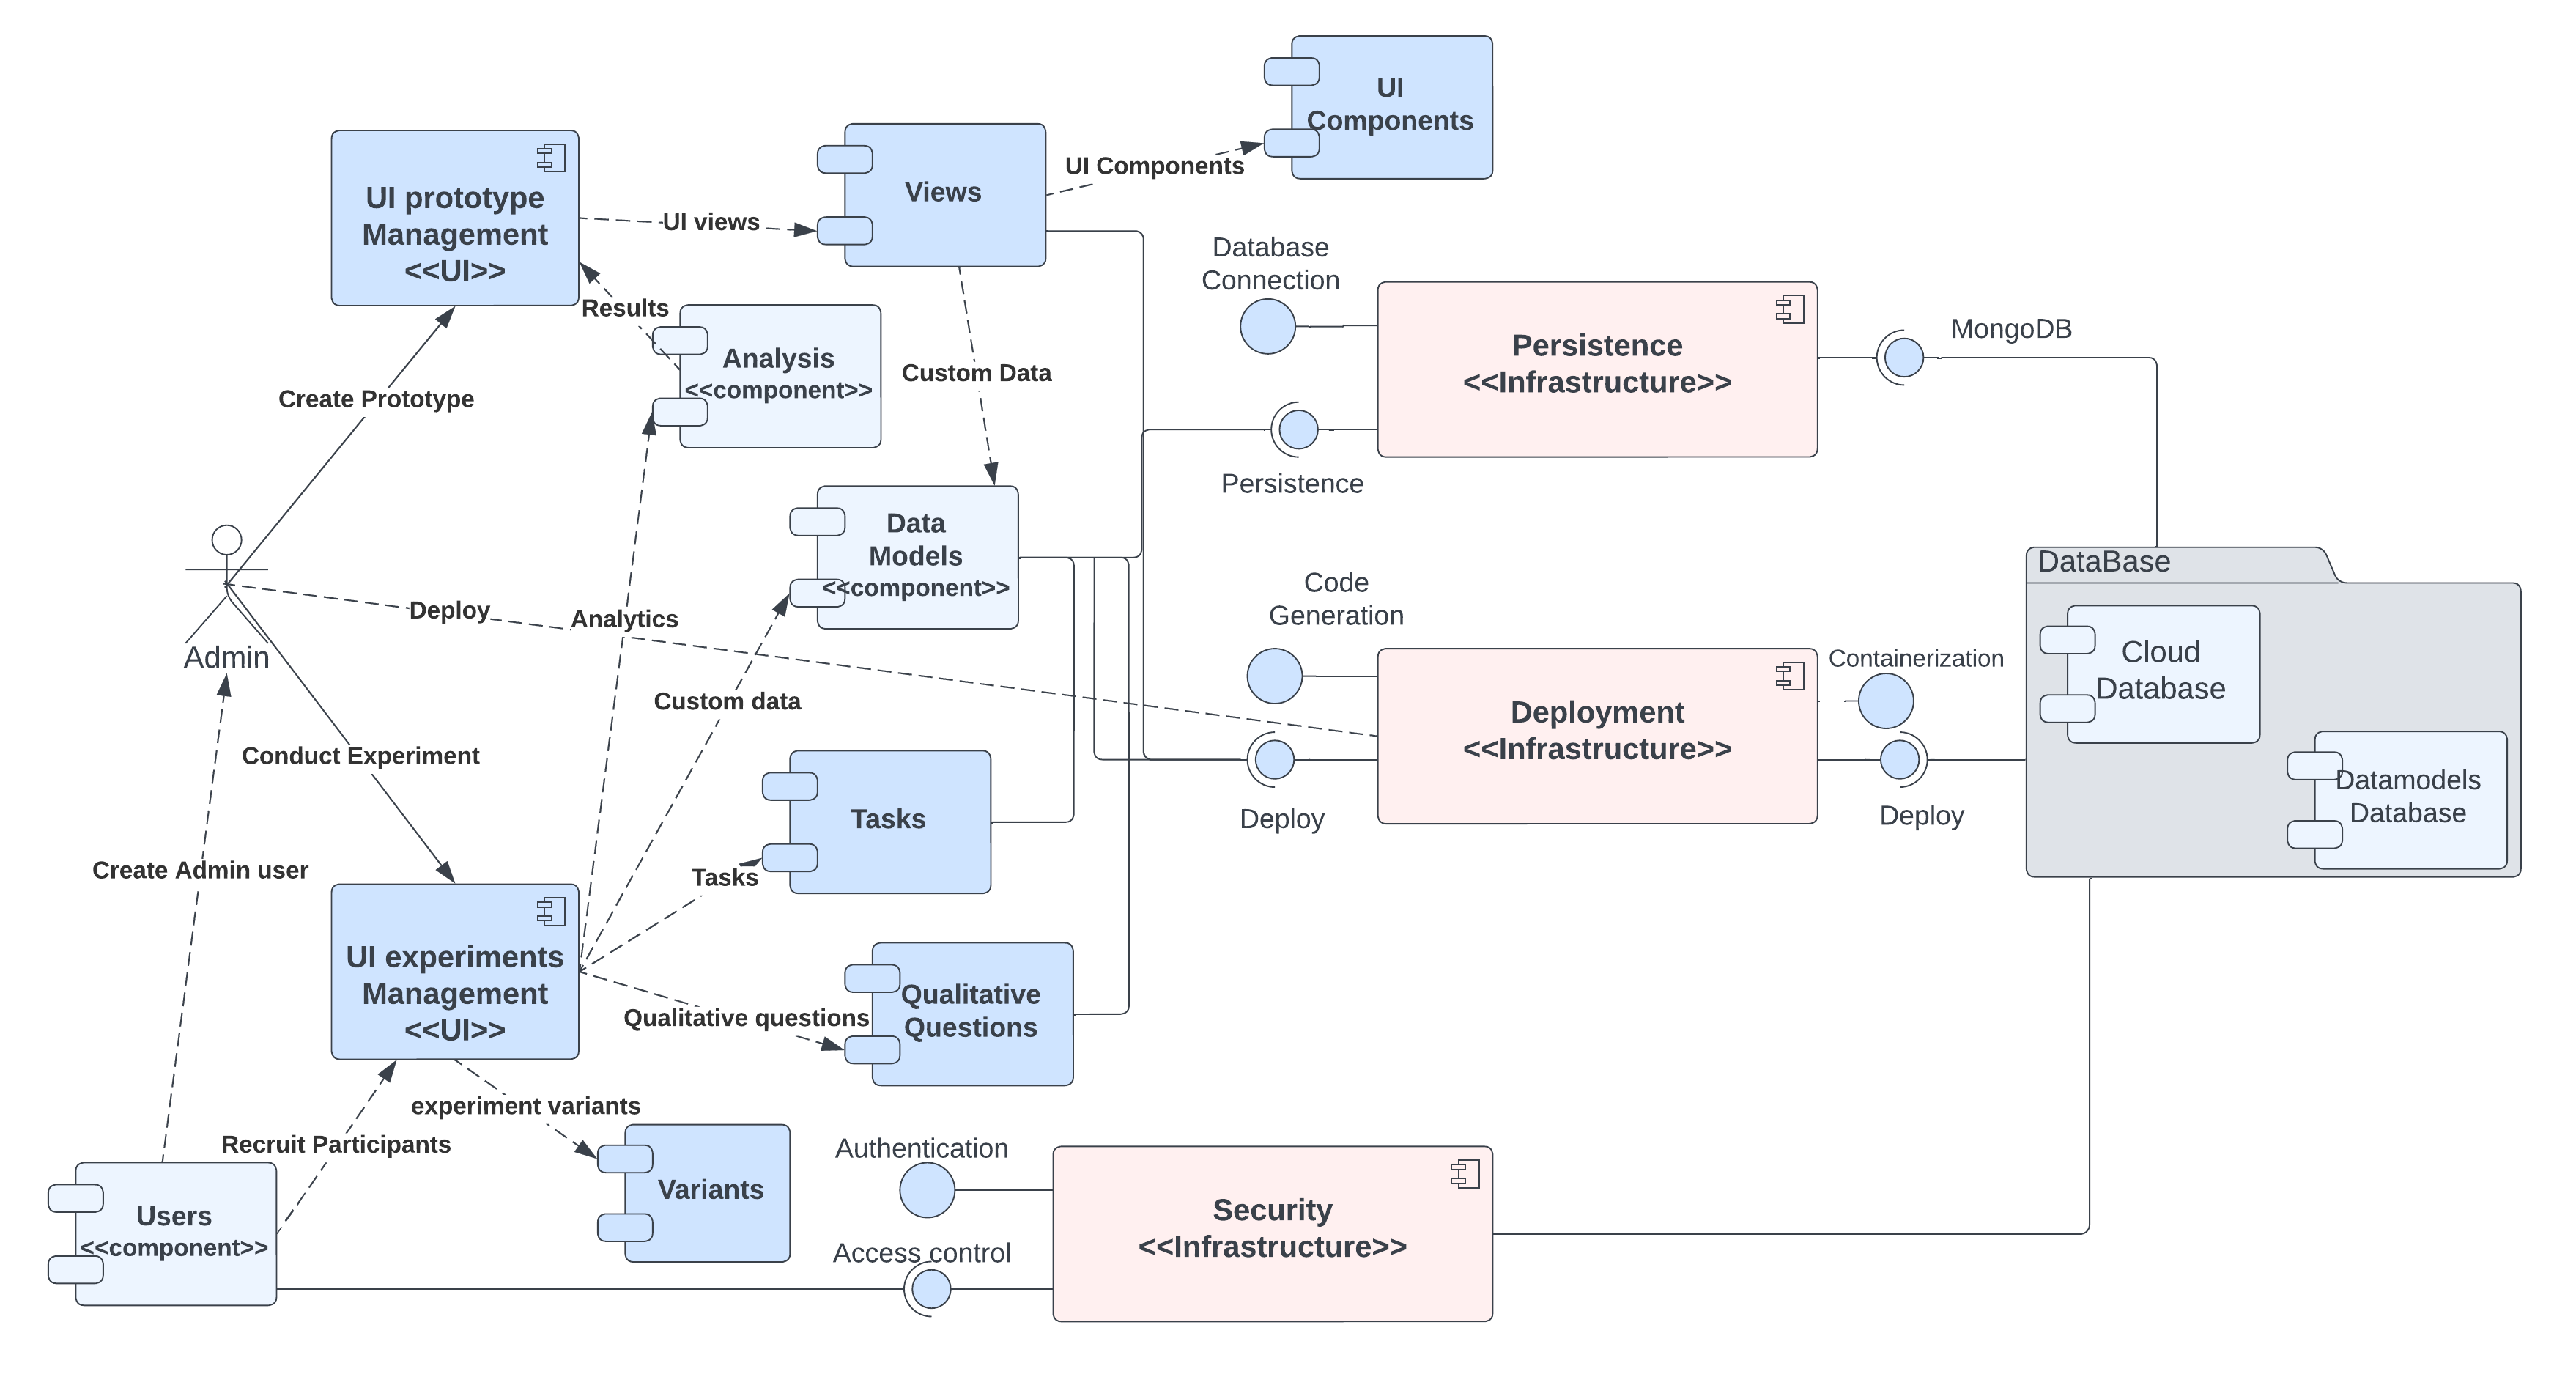
\includegraphics[width=1.1\textwidth]{Component_Diagram.png} 
    \caption[Component Diagram]{Component Diagram of our UI Prototyping tool}
    \label{fig:sc:componentD}
\end{figure}
The component diagram shows the different modules and components of the UI prototyping tool and how they interact with each other during the execution of the tool.
To better understand our component diagram, we explain with the help of a Movie streaming software\footnote{Similar to the famous movie streaming services.}.

As shown in figure \ref{fig:sc:componentD}, the \textit{Users Component} is first used to create an \textit{Admin} user. 
Next, you create a UI prototype using the UI prototype Management with that admin user. 
This component represents the prototyping tool's UI consisting of different screens in a Views component. 
Each screen can contain UI elements (e.g., Buttons, TextBox, Input, etc.) used to navigate different screens.
From our movies example, we create different views like HomePage (which is the starting point of the application), SearchMoviesPage (used to search movies), and ViewPage (view to display various movies), and with the help of \textit{Button} \ac{ui} element navigate to various screens.
It is important to note that the \textit{Data Module component} sends custom data to the \textit{Views component} (e.g., sending different movies to screen ViewPage).
The \textit{Data Module} component is used to store and provide various custom data for displaying them on screens.
Once the UI prototype is ready, the admin user can create UI experiments using the \textit{UI Experimentation Management}.

First, we create an experiment and its different variants (e.g., \textit{ViewExperiment} as an experiment with its variants \textit{GridViewMode} and \textit{ListViewMode} displaying the movies in a grid and list view respectively). 
While creating the variants, we need to specify the percentage used to distribute the participant groups while conducting the experiment (e.g., The variant \textit{GridViewMode} with 40\% means that of the participants 40\% will be allocated to this variant and the rest to \textit{ListViewMode}).
Since our solution approach includes a task-based usability test to get user feedback, the admin user must create various tasks supported by the \textit{Tasks} component (e.g., Navigate to a movie titled ``Transformers'').
With this, we collect participants' quantitative data (like the time to complete the task, the path taken by the participant, and the number of unsuccessful attempts). 
Additionally, the admin user should add qualitative questions to collect qualitative feedback for our solution approach (e.g., ``How satisfied are you with the ease of completing this task?'').
Next, we create the participants for our experiment, which can be done using the \textit{User} component, which provides users for participation.

When the admin users have configured everything, they can start with the experimentation using the \textit{Deployment} infrastructure. 
The deployment infrastructure uses the microservice architecture to deploy all the components as they are independently built. 
The admin should deploy all the components using one button click and ask users to participate in the experiment. 
After the experiment, the admin user can get analytics using the \textit{Analysis} component. 
It provides graphical results of the quantitative analysis of different participants. 
We can also analyze the qualitative analysis using that same component and then decide on the winner variant. 
The results are then passed on to the UI prototype management component, which revises its model for the entire population.  
For the whole application, the \textit{Data Persistance} infrastructure represents the module that manages data persistence in the UI prototyping tool, and \textit{Security} infrastructure is used for access control of the participants and admin users.

\clearpage
\section{Persistance Infrastructure}
\label{sc:section:persistance}
A persistence infrastructure is often necessary for a component diagram to manage a system's data storage and retrieval. 
When a component needs to store data for later use or retrieve data that has been previously stored, a persistence infrastructure can provide the necessary functionality to accomplish this.
Our solution approach uses a persistence infrastructure that provides ``Database connection'' and ``Data persistence'' services for a non-relational MongoDB.
Therefore, the implementation of the persistence infrastructure will be different compared to a traditional relational database. 
MongoDB is a document-oriented database, meaning that data is stored as documents in collections rather than tables with rows and columns.

\paragraph{Database connection}
Our persistence infrastructure provides database connectivity for a non-relational database by using a MongoDB driver or library to interact with the database. 
We install and configure MongoDB on the appropriate servers or cloud-based environments\footnote{Cloud-based environment: \url{https://cloud.mongodb.com/}}.
Then we select a proper driver or library, configure the connection details, and use the driver or library to interact with the database in the components of the system\footnote{How to connect to cloud-based deployed MongoDB instance: \url{https://www.mongodb.com/docs/atlas/connect-to-database-deployment/}}.
Utilizing the driver or library, we interact with the non-relational database in the components of the system. It typically involves defining data models, creating, reading, updating, and deleting documents or records, and querying the database using the appropriate syntax and commands.

\paragraph{Data persistance}
After setting up the necessary drivers or libraries to connect to the MongoDB instance from the components in the system, we define the necessary CRUD (create, read, update, delete) operations for the data models.
These include methods for inserting, updating, deleting, and retrieving data from the database. 
It also provides the necessary validation and error handling for the data models and CRUD operations.\\\\
In summary, when implementing a persistence infrastructure for a non-relational database like MongoDB, we developed the structure and functionality of the database and designed the persistence layer accordingly. 
Therefore, the system can store and retrieve data in an efficient, scalable, and reliable way.

\clearpage
\section{Deployment Infrastructure}
\label{sc:section:deployment}
A deployment infrastructure is necessary for a component diagram to ensure that the system is deployed and running in a secure, scalable, and reliable way. 
A deployment infrastructure is responsible for managing the deployment of components, ensuring that they are running on the appropriate servers or cloud-based environments, and monitoring their performance.
We use a no-code platform and microservice architecture to simplify deployment infrastructure implementation. It allows for creating deployment pipelines and automates many of the processes involved in deploying components.

\paragraph{Code Generation}
We use a no-code approach using code generation to simplify the implementation of our deployment infrastructure by automating many of the tasks involved in deploying the system.
So, we define a set of rules and templates for automatic code generation and generate some reusable components as defined by the UI prototyping management. 
These components' implementation uses templates containing its code (e.g., for a button element defined in the UI prototype, a template is generated containing all its properties and logic).
Then, the code generator takes input data, including configuration files, database schemas, and models of system components and their interactions. 
Finally, the code will be generated using the templates and rules defined in the previous steps, and we will containerize the generated code. 

\paragraph{Containerization}
The deployment infrastructure plays an even more important role in using a microservice architecture. 
It must support the deployment of many independent microservices that may be deployed across multiple servers or data centers (for databases).
From our component diagram, we first identify the system's microservices and their dependencies, such as database components, UI prototyping management, and UI experimentation management. 
It helps determine how the microservices should be deployed and how they should communicate.
Next, we create Docker images for each microservice and its dependencies.
Then, we define docker-compose files\footnote{A Docker Compose file is a YAML file that specifies the microservices, their dependencies, and how they should be deployed and connected.} that describe how the docker containers should be deployed and connected.
Finally, we build the Docker images and deploy them as containers using the docker-compose file. \\\\
In summary, implementing a deployment infrastructure for a microservice architecture can simplify the deployment and management of microservices, making it easier to build and maintain complex systems.

\clearpage
\section{Security Infrastructure}
\label{sc:section:security}
A security infrastructure is essential in a component diagram to protect the system from unauthorized access and attacks. 
By implementing security measures, such as access control, we limit access to sensitive information and functions to only authorized users.
Similarly, authentication is one of the fundamental security mechanisms used to verify the identity of users.
Our security infrastructure, therefore, provides access control and some authentication mechanisms.

\paragraph{Access control}
Access control involves defining policies and rules determining who can access resources under what circumstances.
Therefore we implement access control mechanisms using role-based access control (RBAC) and then allowing or denying access based on those roles or groups.
So, we first identify the roles or groups requiring system access, including participants, administrators, and other users\footnote{This may include different stakeholders like designers, product managers, developers, etc.}. 
Then we define the access rights (e.g., the UI prototyping management should only be accessible to the admin users).
Finally, we implement a mechanism that checks the user roles and then accesses the data or services accordingly. 

\paragraph{Authentication mechanisms}
Authentication involves verifying the identity of users and ensuring that they have the appropriate permissions to access the system.
We provide an authentication mechanism using a password and username. 
It ensures that only authorized users can access our tool.
Moreover, we define some validators for password strength to make sure the passwords are strong.\\\\
In summary, implementing a security infrastructure providing access control and authentication mechanisms for our tool can help prevent unauthorized access and protect sensitive data from being compromised.

\clearpage
\section{UI Experimentation management}
\label{sc:section:experimentation}
In our solution approach, we must have features for creating various UI variants and conducting experiments of A/B testing. 
Therefore, using this component, we allow the admin users to create experiments on the UI as defined in the UI prototype.
It consists of various sub-components for constructing UI variants, assigning participants to experiments, managing participants' tasks, including qualitative questions, and analyzing results. 

\paragraph{Constructing UI Variants}
The UI Variants component represents the different variations of a UI that are used in A/B testing. 
Here, we compare two or more UI variations or variants to determine which performs better regarding user engagement and conversion rates. 
Firstly, the admin user is responsible for creating an experiment and its other variants. 
Then we modify the UI prototype for each variant to have some differences and uniqueness. 
Hence, using our interactive prototyping tool, the admin user should be able to design each variant accurately.
In the end, we have a unique prototype for each UI variant.

\paragraph{Participants Assignments}
An important aspect while experimenting or A/B Testing is the users' participation. 
The admin user is responsible for assigning the participants to their variants. 
Therefore, we need to specify the percentage of participants allocated to an experiment variant during an experiment. 
For our solution approach, we use the between-group study such that different participants test each UI variant so that each person is only exposed to a single variant. 

\paragraph{Task Management}
We need to assign them certain user tasks to get quantitative feedback from the participants. 
It means the admin user must create certain tasks before the start of the experiment.
Our solution approach has a \textit{Tasks} component that provides a feature for creating user tasks for every UI experiment. 
These tasks are built and maintained in our tool by the admin user and are useful while collecting user feedback. 
So, the participants carry out the tasks, and our tool would collect their interaction details (e.g., time taken to finish the task, the path taken by the participant, number of unsuccessful attempts). 

\paragraph{Qualitative Questions}
Since we combine qualitative and quantitative analysis, our solution approach must provide a feature for creating qualitative questions for the participants. 
The \textit{Qualitative questions} component is responsible for providing this feature to the admin user who creates these questions. 
As for the participants, after finishing every task, the participants are asked these questions, and the tool collects the responses. 

\paragraph{Analyze Results}
Every experiment needs to visualize its results, and the visualization component is responsible for providing this feature of analyzing the results of the A/B testing to determine which UI variant performs better. 
This component compares the user engagement and conversion rates for each variant (e.g., time to finish the task, unsuccessful attempts, etc.) and identifies the factors contributing to the performance differences. 
Once we receive the details of the winner variant from this component, the tool sends these details to the original UI prototyping management to iterate and refine the UI variants based on the experiment's results. \\\\
In summary, implementing an experiments management component simplifies the A/B testing, helps improve the effectiveness of the UI, and allows you to manage and track the different interface variations.